% 1999 年全国卷理科第 24 题：角平分线轨迹示意图
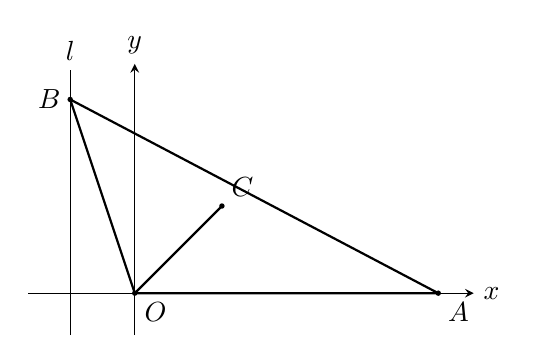
\begin{tikzpicture}[>=stealth, scale=0.82]
  \coordinate (O) at (0,0);
  \coordinate (A) at (4.7,0);
  \coordinate (B) at (-1,3.0);
  \coordinate (C) at (1.35,1.35);

  \draw[->] (-1.65,0)--(5.25,0) node[right] {$x$};
  \draw[->] (0,-0.65)--(0,3.55) node[above] {$y$};
  \draw (-1,-0.65)--(-1,3.45) node[above] {$l$};
  \draw[thick] (B)--(A);
  \draw[thick] (B)--(O)--(A);
  \draw[thick] (O)--(C);

  \fill (O) circle (1.2pt) node[below right] {$O$};
  \fill (A) circle (1.2pt) node[below right] {$A$};
  \fill (B) circle (1.2pt) node[left] {$B$};
  \fill (C) circle (1.2pt) node[above right] {$C$};
\end{tikzpicture}
